\chapter{Metodologia}
\label{cap:metodologia}
Dados os conceitos que envolvem a diferença de desempenho entre a paravirtualização e a virtualização total e os problemas relacionados a interferência entre máquinas virtuais, neste capítulo serão definidas as abordagens que irão dar norte para o desenvolvimento desse trabalho. Desse modo, em um primeiro momento são apresentados os trabalhos relacionados à análise de desempenho em ambientes virtuais, de modo que é definida a abordagem mais adequada. Por fim, são apresentados as espeficações voltadas para ambientes de testes e coleta de dados.
\section{Trabalhos relacionados}
Essa Seção tem como intuito expor alguns trabalhos relacionados à análise de desempenho. Esses trabalhos também servirão de insumo para desenvolvimento do estudo de interferência de desempenho proposto por este trabalho.

No artigo apresentado por \citeonline{koh2007} é feito um estudo de interferência entre aplicações executadas sobre o mesmo \textit{hardware} a partir de duas máquinas virtuais diferentes. Como cargas de trabalho foram escolhidas aplicações do mundo real utilizadas para compressão, compilação de código fonte, e processamento digital, bem como foram utilizadas ferramentas voltadas para testes de desempenho (\textit{benchmark}).

%\footnotetext[1]{AIM Benchmark (http://sourceforge.net/projects/aimbench)}
%\footnotetext[2]{FreeBench ( http://www.freebench.org/ )}
%\footnotetext[3]{LMbench - Tools for Performance Analysis ( http://www.bitmover.com/lmbench/ )}
%\footnotetext[4] {Bzip (http://www.bzip.org/)}
%\footnotetext[5]{Cachebench memory benchmark (http://icl.cs.utk.edu/projects/llcbench/cachebench.html)}
%\footnotetext[6]{Gzip (http://www.gzip.org/)}
%\footnotetext[7]{IOzone Filesystem Benchmark (http://www.iozone.org)}
%\footnotetext[8]{The Persistence of Vision Raytracer (http://www.povray.org)}

Este artigo mostra que duas aplicações, cada uma sendo executada em uma máquina virtual diferente, podem interferir no desempenho da outra. A análise de dados é baseada no cálculo de degradação de desempenho de uma aplicação, para o seguinte conjunto de métricas: média de uso de CPU, \textit{cache hits}, \textit{cache misses}, troca de máquinas virtuais por segundo, bloqueio de operações de entrada e saída por segundo, quantidade de requisição de leitura e escrita por segundo e tempo gasto na leitura e escrita para o disco da máquina virtual. %De maneira geral, a observação feita neste trabalho é que determinadas aplicações podem sofrer mais interferências de outras aplicações que possuem o mesmo uso de tipo de recurso. %O exemplo disso é apresentado na Figura \ref{interference_app}, onde uma aplicação executada soz, sem interferência alcança uma pontuação de 1. Duas aplicações que não interferem uma com a outra alcança uma pontuação perto de 2, como \textit{grep}+\textit{povray}. Já executando \textit{grep}+\textit{grep} a pontuação cai para 0.35 %Por exemplo, uma aplicação A que costuma consumir mais CPU, po{de sofrer mais interferência de uma outra aplicação que possui a mesma característica, do que de uma aplicação que realiza operações mais focadas na escrita de disco. Além disso, é proposto por esse trabalho que com resultados desses desempenhos pode se fazer predição de desempenho de uma aplicação qualquer, a partir de analise matemáticas.

%\begin{figure}[!htb]
%\centering
%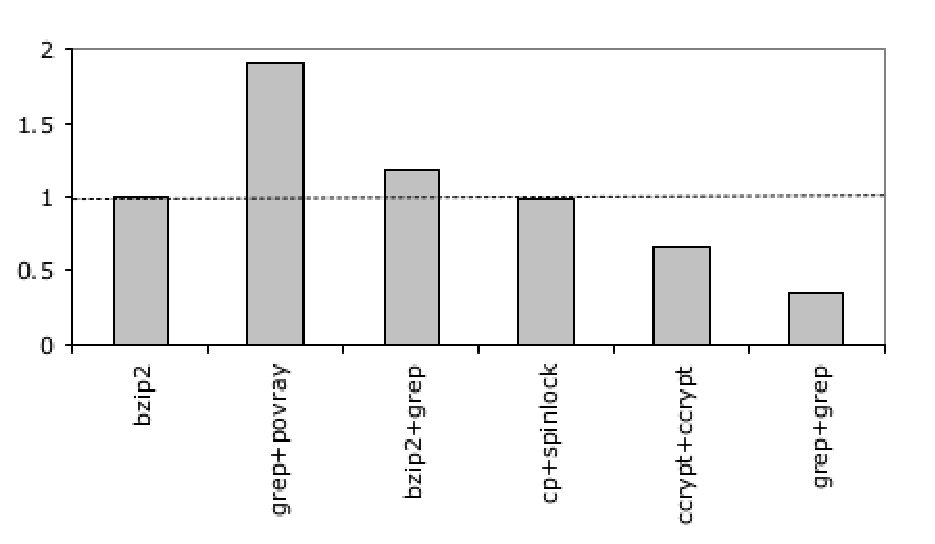
\includegraphics [keepaspectratio=true,scale=0.65]{figuras/interference_aplications.eps}
%\caption{Variação de desempenho para combinações diferentes de aplicações}
%\cite{koh2007}.
%\label{interference_app}
%\end{figure}

Além disso, é mostrado que com resultados desses desempenhos é possível fazer predição de desempenho de uma aplicação qualquer, a partir de análises estatísticas. Dada a quantidade de variáveis, que são as métricas utilizadas para medição de desempenho, as análises estatísticas escolhidas foram a média ponderada com o auxílio da análise de componente principal (PCA) e a análise de regressão linear. Um comparativo entre as análises foi feito de modo que chegou-se a conclusão que análise por média ponderada apresentava uma porcentagem de erro menor. Esse artigo demonstrou que a taxa de erro utilizando o modelo com média pondeerada com o auxílio do PCA se manteve igual, mesmo utilizando outros servidores físicos com configurações diferentes. Entretanto, uma das restrições deste artigo é que o mesmo fora aplicado em aplicações que estavam sendo executadas em duas máquinas virtuais. Desse modo, como trabalhos futuros é proposta a investigação no uso de mais máquinas virtuais, e aplicação de modelos não lineares para predição de desempenho bem como a adição de novos tipos de métricas que envolvam outras características a nível de sistema, tal como desempenho de aplicações de rede.

O artigo de \citeonline{popiolek2012}, disserta sobre a importância de se utilizar métricas nativas (Tabela \ref{metric_tools}) de sistemas  operacionais tais como \textit{Linux} e \textit{Windows} para detecção de gargalos de desempenho. Esse trabalho acaba focando na aferição de operações de entrada e saída, memória e uso de CPU, utilizando ferramentas de \textit{benchmark} para geração de cargas de trabalho. Seus cenários de teste são basicamente variando de uma a seis máquinas virtuais, sendo que o \textit{hypervisor} utilizado é o \textit{KVM}. As análises permitem mostrar a queda de desempenho como um todo quando se tem o aumento do número de máquinas virtuais em execução (Figura \ref{iobound_experiments}). Como trabalho futuros, propõe-se que sejam feitas análise estatísticas afim de comprovar possíveis relações entre as métricas observadas, alem de determinar o limiar que um sistema pode operar sem ter perda significativa no desempenho.
\begin{figure}[!htb]
\centering
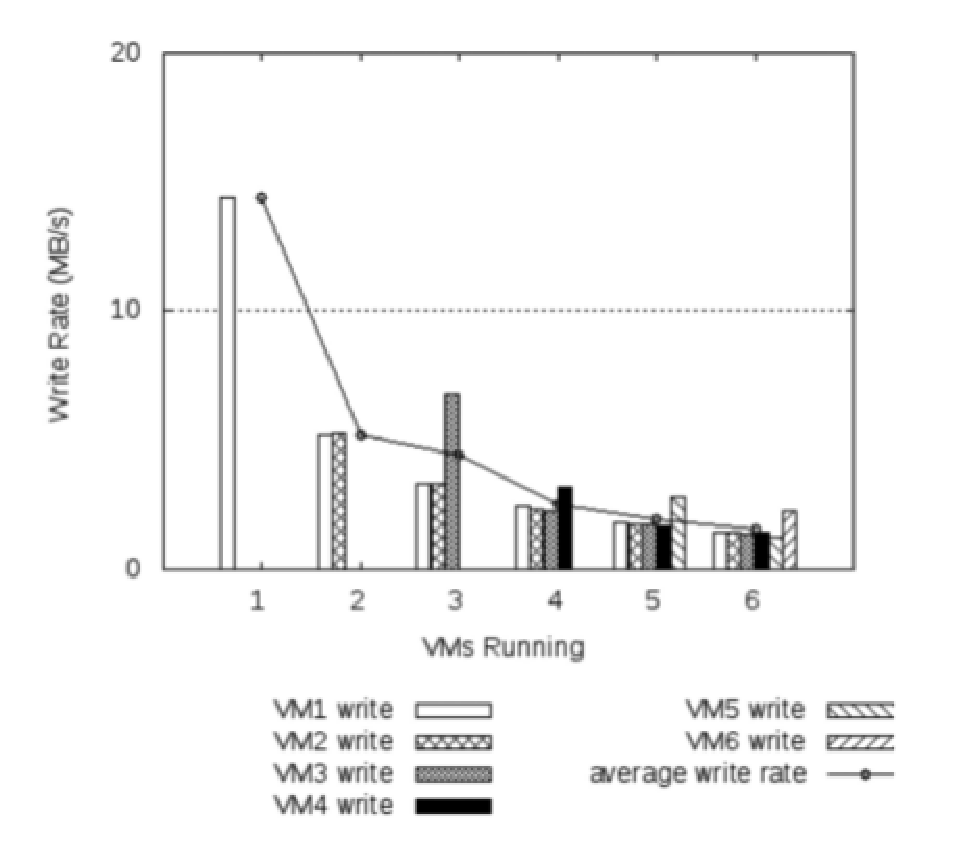
\includegraphics [keepaspectratio=true,scale=0.6]{figuras/iobound_experiments.eps}
\caption{Taxa de escrita em disco para experimentos voltados para E/S.}
\cite{popiolek2012}.
\label{iobound_experiments}
\end{figure}

\begin{table}[!htb]
\centering
\caption{Contadores de desempenho de disco para \textit{Windows} e \textit{Linux} \cite{popiolek2012}}
\label{metric_tools}
\resizebox{1.0\textwidth}{!}{
\begin{tabular}{lllll}
\cline{1-4}
\multicolumn{1}{|l|}{Windows}                & \multicolumn{2}{l|}{Linux}                                             & \multicolumn{1}{c|}{\multirow{2}{*}{Descricão}}                                                                                                  &  \\ \cline{1-3}
\multicolumn{1}{|l|}{Monitor de Desempenho}  & \multicolumn{1}{l|}{iostat}          & \multicolumn{1}{l|}{df}         & \multicolumn{1}{c|}{}                                                                                                                            &  \\ \cline{1-4}
\multicolumn{1}{|l|}{\%Idle Time}            & \multicolumn{1}{l|}{-}               & \multicolumn{1}{c|}{-}          & \multicolumn{1}{c|}{\begin{tabular}[c]{@{}c@{}}Porcentagem de tempo\\  que o disco permanece inativo\end{tabular}}                               &  \\ \cline{1-4}
\multicolumn{1}{|l|}{(Disk Bytes/sec)/ 1024} & \multicolumn{1}{l|}{(rKB/s)+(wKB/s)} & \multicolumn{1}{c|}{-}          & \multicolumn{1}{c|}{\begin{tabular}[c]{@{}c@{}}Número de Kilobytes \\ lidos/escritos por segundo\end{tabular}}                                   &  \\ \cline{1-4}
\multicolumn{1}{|l|}{Disk Transfers/sec}     & \multicolumn{1}{l|}{(r/s)+(w/s)}     & \multicolumn{1}{c|}{-}          & \multicolumn{1}{c|}{\begin{tabular}[c]{@{}c@{}}Número de requisições\\  por segundo completadas\end{tabular}}                                    &  \\ \cline{1-4}
\multicolumn{1}{|l|}{Split IO/sec}           & \multicolumn{1}{c|}{-}               & \multicolumn{1}{c|}{-}          & \multicolumn{1}{c|}{\begin{tabular}[c]{@{}c@{}}Número de requisições por segundo\\  que foram divididas\\ em múltiplas requisições\end{tabular}} &  \\ \cline{1-4}
\multicolumn{1}{|l|}{Free Megabytes}         & \multicolumn{1}{c|}{-}               & \multicolumn{1}{l|}{Disponível} & \multicolumn{1}{c|}{\begin{tabular}[c]{@{}c@{}}Megabytes disponíveis para uso\\  em unidade de armazenamento\end{tabular}}                       &  \\ \cline{1-4}
\multicolumn{1}{|l|}{Avg. Disk sec/Transfer} & \multicolumn{1}{l|}{Await}           & \multicolumn{1}{c|}{-}          & \multicolumn{1}{l|}{Média de tempo para completar uma requisição}                                                                                &  \\ \cline{1-4}
\multicolumn{1}{|l|}{Avg. DIsk Queue Length} & \multicolumn{1}{l|}{avgqu-sz}        & \multicolumn{1}{c|}{-}          & \multicolumn{1}{c|}{\begin{tabular}[c]{@{}c@{}}Média de tamanho de filas de requisições\\  esperando pelo disco rígido\end{tabular}}             &  \\ \cline{1-4}                                             &                                      &                                 &                                                                                                                                                  
\end{tabular}}
\end{table}

Por fim, o artigo de \citeonline{huber2011} tem como intuito prover um modelo genérico de predição de desempenho a partir de determinados fatores que podem interferir na virtualização(Figura \ref{influence_factors}). A idéia é que esse modelo genérico seja aplicável em diferentes tipos plataformas de virtualização. Assim, nesse artigo os experimentos são aplicados nos \textit{hypervisors } \textit{Citrix XenServer 5.5} e \textit{VMware ESX 4.0}. Os fatores categorizados para os experimentos foram: tipo de virtualização, configuração de gerenciamento de recursos e perfis de cargas de trabalho. Para o tipo de virtualização, os experimentos consistem em observar a perda de desempenho ocasionada com a virtualização. Na categoria de configuração de gerenciamento de recursos, são considerados fatores de configuração como número de máquinas virtuais e afinidade de núcleo. E para cargas de trabalho, foram executadas algumas ferramentas de \textit{benchmarking} a fim de se analisar diversas cargas de trabalho. Para o modelo de predição, fora utilizada análise de regressão linear assim como feito em \citeonline{koh2007}. 

\begin{figure}[!htb]
\centering
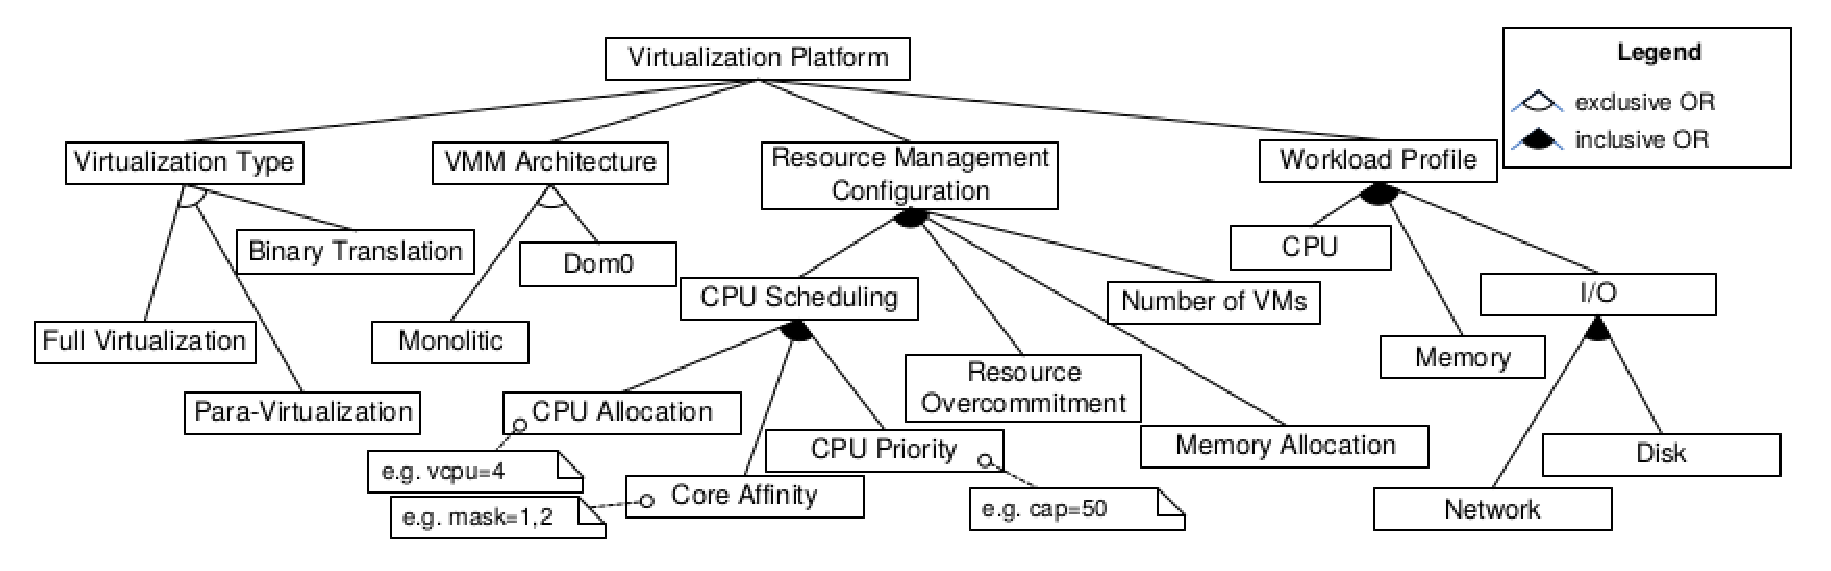
\includegraphics [keepaspectratio=true,scale=0.50]{figuras/factors_influence.eps}
\caption{Fatores que influenciam no desempenho de plataformas virtualizadas}
\cite{huber2011}.
\label{influence_factors}
\end{figure} 

Os artigos de \citeonline{koh2007} e \citeonline{huber2011} tem como ponto em comum o desenvolvimento de mecanismos que possam predizer o desempenho em ambientes virtualizados, uma característica interessante é que \citeonline{huber2011} aplica os mesmos experimentos em \textit{hypervisors} com arquiteturas distintas. Já o artigo de \citeonline{koh2007}, apesar de fazer essa análise em apenas um \textit{hypervisor}, acaba focando na interferência que determinadas aplicações utilizadas no cotidiano, dependendo de sua característica a nível de sistema, podem ocasionar em outras aplicações executadas em máquinas virtuais diferentes, no mesmo servidor físico, trazendo assim um experimento mais próximo do que acontece no mundo real, tornando isso um diferencial desse trabalho. Desse modo, ainda com relação ao artigo de \citeonline{koh2007}, um questionamento que poderia ser feito é com relação a aplicabilidade deste experimento em um outro \textit{hypervisor} com um tipo de virtualização diferente do apresentado no trabalho. Já o trabalho de \citeonline{popiolek2012} é mais voltado para monitoramento, análise de desempenho e detecção de gargalos a partir de métricas nativas do sistema operacional não sendo feito, como nos outros trabalhos, qualquer iniciativa de predição de desempenho.

Dados os trabalhos relacionados apresentados, o de \citeonline{koh2007} foi o que apresentou resultados mais significativos em um nível de detalhamento mais avançado, sendo dessa forma considerado o mais adequado para ser utilizado como insumo para desenvolvimento deste trabalho. Ainda mais, quando se pode verificar a extensibiliidade do trabalho de \citeonline{koh2007} para outro \textit{hypervisor} como o \textit{KVM}. Entretanto, em aspectos metodológicos, esse artigo se demonstrou bastante deficiente, dificultando de certo modo a replicação dos experimentos realizados. Para análise de dados a partir da predição de desempenho, além dos modelos utilizados no trabalho de \citeonline{koh2007}, este trabalho aplica a Regressão Polinomial. No Capítulo tal é feito um comparativo nos resultados obtidos entre os modelos de predição.   %A partir disso, uma outra contribuição deste trabalho se comparado ao de \citeonline{koh2007} é o detalhamento dos experimentos efetuados, de modo que o mesmo possa ser replicado em trabalhos futuros.

%\section{Questão problema}
%Dado que o trabalho de \citeonline{koh2007} apresenta uma análise de interferência de desempenho utilizando o \textit{XEN}, que é um %\textit{hypervisor} conhecido por utilizar a paravirtualização para provimento de máquinas virtuais, este trabalho visará responder %a seguinte questão:

%\textit{ Qual  grau de interferência entra máquinas virtuais, executando sob o mesmo servidor, utilizando o \textit{KVM} como \textit{hypervisor}, que implementa a virtualização total?  }
 
%Tendo essa questão como ponto de referência, a proposta deste trabalho é a aplicar o mesmo estudo de interferência entre máquinas /%virtuais feito no trabalho de \citeonline{koh2007}, de modo que sejam comparados grau de interferência entre as duas técnicas de %virtualização existentes: paravirtualização e virtualização total.
%\subsection{Hipótese}
%A partir da questão problema definiu-se a seguinte hipótese que irá motivar a realização deste trabalho:

%\begin{itemize}
    %\item \textit{H1}: O estudo de interferência entre aplicações executadas em ambientes virtualizados proposto por \citeonline{koh2007} é aplicável em outros tipos de plataforma de virtualização 
    
	%\item \textit{H1}: O \textit{XEN}, por utilizar a paravirtualização como técnica de virtualização, apresenta menor interferência entre máquinas virtuais do que o \textit{KVM}. Como explicado no capítulo \ref{sec:infraestrutura}, a paravirtualização tende a possuir um ganho de desempenho se comparado com  virtualização total. Comparando os resultados do trabalho de \citeonline{koh2007}, feitos com \textit{hypervisor} \textit{XEN}(paravirtualização), com os resultados de interferência provenientes de um \textit{hypervisor} \textit{KVM}(Virtualização total), é uma ótima oportunidade de verificar a diferença de desempenho entre os dois tipos de virtualização.
	%\item \textit{H2}: O modelo de prediçã proposto por \citeonline{koh2007} man
	%\item \textit{H2}: O modelo de predição proposto por \citeonline{koh2007} é aplicável em um ambiente com características distintas de \textit{hardware} e de plataforma de virtualização. Em seu trabalho, \citeonline{koh2007} é relatado que esforços já estavam sendo empreendidos para verificar a portabilidade do seu estudo de interferência para outros tipos de ambientes de \textit{hardware}. Entretanto, não foi encontrado qualquer tipo de evidência em algum trabalho futuro que apresente a aplicação deste estudo em outro tipo de ambiente. Dessa forma, com outro tipo de \textit{hypervisor} (\textit{KVM}) e com configurações de \textit{hardware} apresentados no capítulo \ref{cap:resultados}, é interessante verificar aplicabilidade deste experimento para outros tipo de plataforma tanto no quesito de \textit{hardware} quanto de virtualização. 
	%\item \textit{H3}: Com esse mecanismo de predição de desempenho é possível propor uma nova distribuição de aplicações em um ambiente com múltiplas máquinas virtuais.  %reformular
%\end{itemize}
	
\section{Ambiente de Testes}\label{sec:ambiente_teste}
Para o estudo proposto por este trabalho foi definido um  ambiente de testes que consiste no uso de máquinas virtuais com aplicações voltadas para realização
de testes de \textit{benchmark}. Tais aplicações foram definidas a partir do trabalho de \citeonline{koh2007}, tendo essas sido escolhidas visando o estresse de vários aspectos de sistema e de \textit{hardware}. Com a infraestrutura de computação em nuvem implementada com o \textit{OpenNebula} foi possível a criação desses ambientes de testes em máquinas virtuais criadas remotamente. As máquinas virtuais possuíam, como configuração, sistema operacional \textit{Centos 7}, espaço em disco de 15GB e 1GB de memória \textit{RAM}. Em um primeiro momento as aplicações foram instaladas e testadas de modo que se pudesse observar quais são os comandos utilizados para funcionamento das mesmas, em seguida foram criados \textit{snapshots} das máquinas virtuais com o auxílio provido pelo \textit{OpenNebula}. 

Assim era possível criar, destruir e efetuar quaisquer tipos de testes com relativa comodidade. Entre as aplicações escolhidas estão típicas provedoras de \textit{stress} computacional no cotidiano, tais como compilação de código fonte, compressão e encriptação de arquivos e processamento de imagens. Há também ferramentas voltadas para geração de testes de \textit{benchmark} tais como \textit{Cachebench} e \textit{AIM Benchmark suite}. A seguir é feita uma breve descrição das ferramentas utilizadas.

\begin{itemize}
\item \textit{Add\_double} \footnotemark[5]                                                                                                                               é um dos vários programas de testes de carga existentes no \textit{AIM benchmark suite}. É responsável por medir operações de adição de dupla precisão.

\item \textit{Bzip2} \footnotemark[6] e \textit{Gzip} \footnotemark[7] são aplicações típicas para compressão e descompressão de arquivos. Com uso de arquivos grandes é possível gerar cargas de trabalhos usando essas ferramentas.

\item \textit{Ccrypt} \footnotemark[8] é uma ferramenta de código aberto voltada para encriptação e desencriptação de arquivos. Foi desenvolvido com o intuito de substituir a aplicação padrão do \textit{unix}, o \textit{crypt}.

\item \textit{Cachebench} \footnotemark[9] é uma ferramenta de \textit{benchmark} de código aberto desenvolvida para avaliar o desempempenho do subsistema de memória. Atualmente é integrado \textit{LLCbench} (\textit{Low-Level Characterization Benchmarks}).

\item \textit{Cat} e \textit{Grep} são comandos padrões em sistemas \textit{Linux} que são responsáveis por gerar requisições de leitura no disco. \textit{Cat} é reponsável por mostrar conteúdo de arquivos bem como combina-los e criar outros novos. Enquanto que \textit{Grep} é utilizado para busca de palavras em arquivos texto.

\item \textit{cp} e \textit{dd} são outros comandos padrões em sistemas \textit{Linux}, neste caso, responsáveis por gerar atividades voltadas para escrita de disco. \textit{cp} é utilizado para copiar arquivos e diretórios. O comando \textit{dd} é utilizado para criação de imagens e cópias de arquivos.

\item \textit{Iozone} \footnotemark[10] é uma ferramenta de \textit{benchmark} utilizada, voltada para testes de operações de disco, tais como leitura e escrita.

\item \textit{Make} é um comando nativo em sistemas operacionais \textit{Linux}, responsável por automatizar um conjunto de procedimentos, principalmente  a compilação de programas grandes que possuem vários arquivos com códigos fontes. 

\item \textit{Povray} \footnotemark[11] é uma ferramenta de codigo aberto voltada para processamento de imagens com gráficos 3-D.

\end{itemize}

\footnotetext[5]{AIM Benchmark (http://sourceforge.net/projects/aimbench)}
\footnotetext[6] {Bzip2 (http://www.bzip.org/)}
\footnotetext[7]{Gzip (http://www.gzip.org/)}
\footnotetext[8]{Ccrypt (http://ccrypt.sourceforge.net/}
\footnotetext[9]{Cachebench memory benchmark (http://icl.cs.utk.edu/projects/llcbench/cachebench.html)}
\footnotetext[10]{IOzone Filesystem Benchmark (http://www.iozone.org)}
\footnotetext[11]{The Persistence of Vision Raytracer (http://www.povray.org)}

%Além das ferramentas já mostradas outras aplicações foram utilizadas no trabalho de \citeonline{koh2007}: \textit{Spinlock}, \textit{CacheBuster} e \textit{Analyser}.

\section{Coleta de dados} 
Dada a configuração do servidor apresentado no Apêndice \ref{sec:infraestrutura}, um dos receios era de que os testes de \textit{benchmark} feitos não fossem suficientes para apresentarem interferência entre as máquinas virtuais, desse modo optou-se por dividir a coleta de dados em três experimentos práticos de modo que, nos dois primeiros experimentos fossem verificadas as interferências entre os diversos tipos de aplicações. Assim, para cada experimento foi definido objetivos específicos a serem alcançados.
%A coleta de dados foi efetuada a apartir da realização de três experimentos práticos. Para cada experimento foi definido objetivos específicos a serem alcançados.%

O primeiro experimento teve como objetivo verificar a existência da interferência entre máquinas virtuais no servidor físico utilizado, sendo neste experimento executado com poucas ferramentas dado que os resultados eram mais voltados para verificação da interferência e motivação da continuidade do trabalho em si do que para uma análise mais profunda. O segundo experimento teve como objetivo verificar a variação de interferência para o conjunto completo das ferramentas já apresentadas sendo construída uma matriz \textit{n x n} com todas as possibilidades. O terceiro experimento, teve como foco a avaliação da interferência para diversos tipos de características a níveis de sistema tais como média de utilização de \textit{CPU} e \textit{leitura e escrita de disco por segundo}, por exemplo. Sendo os resultados desse terceiro e último experimento utilizados como insumo para análise de dados apresentada neste trabalho.% A apresentação dos dados referentes a cada experimento foi baseada nos resultados apresentados no trabalho de \citeonline{koh2007}, visando assim um comparativo dos resultados encontrados para os dois diferentes tipos de virtualizaçaõ: paravirtualização e virtualização total.

\subsection{Cálculo da Interferência}
Os procedimentos adotados para o cálculo da interferência seguem os propostos no trabalho de \citeonline{koh2007}. Desse modo, duas máquinas virtuais, com as especificações e aplicações de \textit{benchmark} apresentadas na Seção \ref{sec:ambiente_teste}, são criadas em um servidor utilizando \textit{hypervisor} \textit{KVM}. Cada máquina virtual, denominadas \textit{'dom1'} e \textit{'dom2'} respectivamente, executa uma das aplicações de \textit{benchmarking}. 

Uma aplicação executando em \textit{dom1} é chamada de aplicação \textit{foreground}, e a que estiver executando em \textit{dom2} é a aplicação \textit{background}. Por questões de notação uma aplicação \textit{foreground} executando contra uma aplicação \textit{background} é denotada como F@B. Um dos procedimentos adotados é garantir que a aplicação \textit{background} mantenha sua execução até que a aplicação \textit{foreground} termine. Para o segundo e terceiro experimento cada aplicação é executada de modo que seja tanto \textit{background} quanto \textit{foreground}, sendo construída dessa forma uma matriz \textit{n x n} com todos os possíveis resultados. %Destaca-se os dados referentes a interferência são mensurados em uma aplicação \textit{foreground}.

A fim de observar o quanto o desempenho é afetado pela interferência gerada por uma aplicação executada em outra máquina virtual, é feita a medida da degradação a partir do desempenho padrão de uma aplicação, essa medida denomina-se pontuação normalizada. Assim, para calcular a pontuação normalizada de uma aplicação, primeiro é definida a pontuação de desempenho inativa que é a pontuação de uma aplicação quando executada contra uma máquina virtual inativa, ou seja sem nenhuma aplicação executando. Então, em seguida é feito o cálculo da pontuação normalizada de uma aplicação F contra B, dividindo a pontuação de desempenho de F contra B pela pontuação de desempenho inativa de F. Assim define-se NS(F@B), como sendo a pontuação normalizada de F contra B,

\begin{equation}
\label{eq:degradation}
NS(F@B) = PontuaçãoDesempenho(F@B)/PontuaçãoDesempenho(F@Inativo)
\end{equation}

A partir disso, é feito cálculo do desempenho combinado de duas aplicações, F e B, em cada máquina virtual.

\begin{equation}
\label{eq:combined}
NS ( F + B ) = NS ( F @ B ) + NS ( B @ F )
\end{equation}
Sendo NS(F@B) e  NS(B@F) medidos em dois testes separados. Para medida de desempenho, nos dois primeiros primeiros experimentos são utilizadas as pontuações geradas pelas próprias aplicações. Entretanto, algumas aplicações, aquelas que não são voltadas para \textit{benchmark}, não geram pontuações explícitas. Para essas aplicações, fora definido como o inverso do tempo necessário para sua execuação, como pontuação de desempenho. Na tabela \ref{table-aplications} é apresentado o maior recurso utilizado bem como a medida de desempenho utilizada para cada ferramenta. Para o terceiro experimento as pontuações utilizadas são métricas de desempenho a nível de sistema.

\begin{table}[!htb]
\centering
\caption{Aplicações utilizadas para geração de cargas e trabalho}
\label{table-aplications}
\begin{tabular}{|l|c|c|}
\hline
Nome        & \multicolumn{1}{l|}{Maior Recurso Utilizado} & \multicolumn{1}{l|}{Medida de Desempenho} \\ \hline
Add\_double & CPU                                          & Pontuação                                  \\ \hline
Bzip2       & Misto                                        & Tempo                                      \\ \hline
Cat         & Disco                                        & Tempo                                      \\ \hline
Cachebench  & Memória                                      & Pontuação                                  \\ \hline
Ccrypt      & Misto                                        & Tempo                                      \\ \hline
Cp          & Disco                                        & Tempo                                      \\ \hline
Dd          & Disco                                        & Tempo                                      \\ \hline
Grep        & Disco                                        & Tempo                                      \\ \hline
Gzip        & Misto                                        & Tempo                                      \\ \hline
Iozone      & Disco                                        & Pontuação                                  \\ \hline
Make        & Misto                                        & Tempo                                      \\ \hline
Povray      & Misto                                        & Tempo                                      \\ \hline
\end{tabular}
\end{table}

Dessa forma, uma pontuação normalizada(F@B) próxima ou igual a 1 é um resultado que indica que o desempenho de uma aplicação \textit{F} contra \textit{B} sofreu baixa degradação.

%Para observar o grau de interferência ocasionada por uma aplicação que está sendo executada em outra máquina virutal, é feito um cálculo  de degradação a partir da pontuação de desempe
\subsection{Métricas de desempenho a nível de sistema}
No trabalho de \citeonline{koh2007} são utilizadas métricas de desempenho a nível de sistema ( denominadas \textit{System-level Workload Characteristics}) de forma a analisar melhor o grau de interferência em diversos aspectos de sistema na máquina virtual. Segundo \citeonline{koh2007}, o fato desse tipo de métrica de desempenho ser independente de qualquer tipo de microarquitetura subjacente, garante que seja possível ser feitas comparações através dos diferentes tipos de servidores físicos.

No trabalho de \citeonline{koh2007} essas métricas são obtidas através de um \textit{hypervisor} instrumentalizado, ou seja no próprio \textit{hypervisor} há mecanismos responsáveis pela coleta dessas métricas de modo que elas são obtidas de fora da máquina virtual, possibilitando assim que a interferência da coleta seja praticamente nula. A partir disso, fora feita uma investigação de como o \textit{hypervisor} utilizado, o \textit{KVM}, ou a plataforma em nuvem \textit{OpenNebula} poderia prover essas métricas sem que fosse necessário qualquer tipo de interferência na máquina virtual para coleta desses dados.

Para o \textit{KVM} chegou-se a ferramentas como o \textit{iperf-kvm} e \textit{kvm-stat}. Entretanto, as informações apresentadas por essas ferramentas não eram claras e, para o caso do \textit{kvm-stat}, não detalhava por máquina virtual e sim para  \textit{hypervisor} inteiro. Mesmo no \textit{OpenNebula} as informações apresentadas consistiam em uso de espaço em disco, memória utilizada e quantidade de \textit{CPU} alocado por máquina virtual, não sendo essas informações relevantes para o estudo proposto. Assim, a abordagem escolhida foi o uso de uma ferramentas típica para monitoramento de desempenho: \textit{iostat} para operações de disco e o \textit{mpstat} para \textit{CPU}. %o \textit{Munin} em conjunto com o \textit{Cachegrind} e o \textit{Virsh}. A seguir são apresentadas as métricas coletadas neste trabalho.

\begin{itemize}
\item \textbf{Porcentagem de uso do \textit{CPU}}(\textit{cpuutil}): Porcantagem de utilização de \textit{CPU} durante a execução de uma aplicação. É obtida através da aplicação \textit{mpstat}.

\item \textbf{Requisições de escrita e leitura de disco por segundo }(\textit{writes\_issued, reads\_issued}) e \textbf{Tempo gasto para escrita e leitura do disco}(\textit{time\_writing, time\_reading}): Quantidade de requisições no disco e o tempo para operações de escrita e leitura são bons indicadores de operações de entrada e saída. Esses valores são coletados utilizando o \textit{iostat}.

\end{itemize}

\subsection{Procedimentos experimentais}
Um dos impasses encontrados no desenvolvimento deste trabalho foi executar os mesmos procedimentos feitos por \citeonline{koh2007}, dado que não fica tão explícito quais foram os caminhos adotados para execução de cada aplicação ou ferramentas de \textit{benchmark}. Dessa maneira, fora necessário definir experimentalmente os procedimentos a serem adotados para geração estresse computacional e coleta de dados. De maneira geral, cada ferramenta era executada 15 vezes, em cada execução o tempo de execução ou a pontuação alcançada (para ferramentas que tinham pontuações explícitas) era coletado. Alcançada a quantidade de 15 execuções era calculada uma média dos dados coletados.

Inicialmente foi definido um número de 30 execuções por ferramentas (uma amostragem de 30 valores). Entretanto, principalmente no segundo experimento, a estimativa de tempo para execução de todas ferramentas se mostrou demasiadamente grande. Dessa forma, cogitou-se o uso de 10 ou 15 valores. De modo a chegar a um valor adequado para amostragem, levando se conta a quantidade o tempo necesário para essa quantidade. Calculou-se o desvio padrão das ferramentas \textit{Make} e \textit{Bzip} para 10, 15 e 30 valores de amostragem, a fim de verificar a diferença de dispersão entre esses valores. A tabela \ref{desvio} apresenta esses resultados.     

\begin{table}[!h]
\centering
\caption{Desvio Padrão para diferentes quantidades de valores para \textit{Povray} e \textit{Make}}
\label{desvio}
\begin{tabular}{|l|c|l|l|}
\hline
Ferramenta            & \multicolumn{1}{l|}{Quantidade de Valores} & Desvio Padrão  & Média         \\ \hline
\multirow{3}{*}{Make} & 10                                         & 0.993032191489 & 44.5126       \\ \cline{2-4} 
                      & 15                                         & 0.436379367501 & 44.3846666667 \\ \cline{2-4} 
                      & 30                                         & 0.379019873315 & 44.3230666667 \\ \hline
\multirow{3}{*}{Gzip} & 10                                         & 0.394128701484 & 31.9069       \\ \cline{2-4} 
                      & 15                                         & 0.229156361673 & 32.0740666667 \\ \cline{2-4} 
                      & 30                                         & 0.249032463378 & 32.1289333333 \\ \hline
\end{tabular}
\end{table}

A diferença do desvio padrão para uma amostragem entre 15 e 30 valores foi considerada irrelevante se comparada com a média alcançada dos resultados. O desvio padrão para uma amostragem de 10 valores mostrou uma dispersão mais elevada, mesmo assim ainda irrelevante a diferença se comparada com a média, mas visando uma margem mas segura de erro, acabou-se definido o uso de uma amostragem de 15 valores. 

Para geração de carga de trabalho a partir das ferramentas selecionadas, alguns procedimentos foram definidos empiricamente, principalmente paras aplicações utilizadas no cotidiano. A seguir são descritos alguns procedimentos adotados para cada ferramenta selecionada.

Para a coleta de dados referentes às métricas de desempenho a nível de sistema, foi definido uma coleta de 300 valores por cada métrica. 
\begin{itemize}
\item \textit{Add\_double}: A única opção para execução dessa ferramenta de \textit{Benchmarking} é a quantidade de tempo que é executada. Foi escolhido um tempo de 30 segundos.

\item \textit{Bzip2, cp, cat, gzip}: Para essas ferramentas foi definido o uso de um arquivo com tamanho de 3 \textit{GB} ( o triplo da memoria da máquina virtual) de modo que se evitasse o efeito de \textit{cache} pela memória. Desse modo, os comandos \textit{cat} e \textit{cp} geravam cargas a partir da geração de cópias desse arquivo. Aplicações \textit{Bzip2} e \textit{gzip}, efetuavam a compreensão desse arquivo com a opção \textit{--best}.

\item \textit{Cachebench}: Possui diferentes tipos de testes de \textit{benchmark} para o sistema de memória, sendo executados para tamanhos variáveis de alocação de memória. É executado com as opções: \textit{-b} ( \textit{Read/Modify/Write benchmark}), \textit{-x0}, \textit{-m24}, \textit{-d1}( 1 segundo por iteração), \textit{-e1}(1 repetição do teste por tamanho de alocação da memória) . Como resultado é considerado apenas o valor da taxa de transferência em \textit{MB/s} apresentado para o maior tamanho de alocação de memória que a ferramenta suporta.

\item  \textit{Ccrypt, grep}: Para essas ferramentas foi utilizado um arquivo de 2\textit{GB}, gerado com números \textit{randômicos} a parir de \textit{/dev/random}. Com \textit{Ccrypt} é efetuada a encriptação do arquivo, com o \textit{grep} é feita uma busca pelo número \textit{'123'}.

\item \textit{Iozone}: Essa ferramenta foi executada de modo que se efetuasse os testes de leitura e escrita no modo sequencial e rândomico.

\item \textit{Make}: Para geração de carga foi efetuada a compilação do código fonte da versão mais recente do \textit{apache} \footnotemark[12]                                                                                                                              . Coletado o tempo para execução da compilação, a mesma é desfeita para que em seguida seja executada novamente, obtendo assim a quantidade de valores necessária para o cálculo da média.

\item \textit{Povray}: Possui um módulo próprio para execução de testes de \textit{benchmark}. O próprio módulo de \textit{benchmark} já contabiliza o tempo de execução dos ceńarios de processamento de imagens da ferramenta. 

\end{itemize}

Para coleta de dados de dados foi construídos \textit{scripts}, utilizando a linguagem \textit{Python} \footnotemark[13]                                                                                                                               com a quantidade de execução bem como os comandos utilizados para cada aplicação e ferramenta de \textit{benchmark}, de modo a garantir mais comodidade na obtenção dos dados. Esses \textit{scripts} estão disponíveis via repositório remoto \footnotemark[14].


\footnotetext[12]{http://www.apache.org/}
\footnotetext[13]{https://www.python.org/}
\footnotetext[14]{https://github.com/MaxAlmeida/TCC-SCRIPTS-MONITORING}

\section{Análise de dados}

A análise dos dados obtidos referentes às métricas de desempenho e às pontuações normalizadas obtidas pelas aplicações foi baseada no uso de técnicas de análise multivariada. A análise multivariada consiste em um conjunto de técnicas estatísticas que tem como intuito dar a possibilidade de inferir padrões ou explicaçoes para um experimento com uma grande quantidade de dados. Sua área de atuação envolve \cite{johnson1988}:
\begin{itemize}
  \item \textbf{Redução de dados ou simplificação estrutural}: O fenômento ou experimento estudado é representado o mais simples possível sem que haja perda de informação valiosa. Dessa forma, espera-se que a interpretação, com os dados reduzidos, seja facilitada.
  
  \item \textbf{Ordemanemto e Agrupamento}: Os dados obtidos são agrupados de acordo com as semelhanças existentes em suas características. Para isso, podem ser necessárias a criação de classificações, dada as características dos dados, bem definidas.
  
  \item \textbf{Investigação de dependência entre as variáveis}: Trata de verificar a relação (independência ou dependência) entre todas as variáveis e como elas acontecem.
  
  \item \textbf{Predição}: As relações entre as variáveis devem ser determinadas com o intuito de predizer os valores de uma ou mais variáveis na base da observação de outras variáveis.
  
  \item \textbf{Construção e Teste de Hipótese}: Hipóteses estatísticas formuladas em função de dados multivariados são testadas. Isso pode ser utilizada para validar suposiçoes ou reforçar convincçoes anteriores.
\end{itemize}

Dessa forma, neste trabalho as técnicas de análise multivariada foram aplicadas com o intuito de predizer o desempenho das aplicações. As técnicas utilizadas foram média ponderada com o auxílio da análise por componente principal (PCA), Regressão Linear e Regressão Polinomial. Destaca-se que a média ponderada não é uma técnica de análise multivariada mas ainda assim fora feito o uso, para agrupamento dos dados, da análise por componente principal. Para realização da análise por componente principal foi utilizada a ferramenta \textit{Scilab} \footnotemark[15] com o auxílio da biblioteca \textit{FACT} \footnotemark[16]. Já para a análise de regressão linear e polinomial foi utilizada uma ferramenta de análise statística chamada \textit{R} \footnotemark[17].

\footnotetext[15]{http://www.scilab.org/}
\footnotetext[16]{https://atoms.scilab.org/toolboxes/FACT/0.9}
\footnotetext[17]{https://www.r-project.org/}


De maneira geral, escolheu-se uma aplicação U a partir do conjunto de aplicações definidos anteriormente. Em seguida, ao utilizar o restante das aplicações como um conjunto de referência (B1, B2, ..., Bn), foi feita a predição da pontuação normalizada de U contra as outras aplicações (i.e, NS(U@B1), NS(U@B2), ... NS(U@Bn)), das aplicações contra U (i.e, NS(B1@U),
NS(B2@U), ... NS(Bn@U)) e de U contra ele mesmo (NS(U@U)). Assim, para cada técnica aplicada, foi comparado a pontuação predita com a pontuação real medida. Para avaliação desse comparativo são calculados a média, mediana e o maior erro da predição obtido, onde o cálculo do erro da predição é feito pela equação \ref{eq:predict_error}. Esse procedimento foi feito com todas as aplicações definidas.  
\begin{equation}
\label{eq:predict_error}
\textrm{Erro da predição} = \frac{|\textrm{Pontuação real - Pontuação predita}|}{\textrm{Pontuação real}}
\end{equation}
\subsection{Método da Média Ponderada}
O método da média ponderada é baseado na similaridade entre duas aplicações. Dessa forma, para calcular a similaridade, primeiro é feito o cálculo da distância dos vetores de métricas de desempenho de duas aplicações. Dada o número de dimensões desse vetor ( 5 métricas de desempenho a nível de sistema), foi aplicada uma análise de componente princiapl ( PCA ) de modo que se reduzisse a dimensionalidade dos dados sem perda significativa.

Assim, embora as \textit{p} variáveis de um vetor de dados sejam necessárias para reproduzir a total variabilidade de um sistema, frequetemente muito dessa variabilidade pode ser representada por uma pequena quantidade \textit{k} de componentes principais. Dessa forma, os \textit{k} componentes principais podem substituir  as \textit{p} variáveis iniciais, reduzindo o conjunto de dados necessários para a análise \cite{johnson1988}.

Uma vez que os dados coletados foram convertidos pela análise de componentes principal, foi feita a escolha dos componentes que representam a maior variabilidade desses dados. Com isso, através dos dados obtidos, foram escolhidos três componentes que representam 94\% da variança total ( Cada componente representa 53,8\%, 24\%, 16,3\% da variança, respectivamente).

Para cálcular a predição da pontuação de U@Bn, adota-se o seguinte procedimento apresentado no trabalho de \citeonline{koh2007}. Primeiro, em cima dos dados transferidos para PCA, foi calculada a distância euclidiana do ponto desejado, U@Bn, para todos os resultados de \textit{benchmark} obtidos e então foram escolhidos os N pontos de dados mais próximos e definidos como um conjunto dos mais próximos. A Tabela \ref{tab:distance} apresenta, de forma resumida, as distâncias de todos os possíveis resultados. Dessa forma, como exemplo, o ponto mais próximo de Crypt @ Bzip2 seria Gzip @ Gzip que possui uma distância no valor próximo de 0.57.

\begin{table}[H]
\centering
\caption{Distâncias entre todos os resultados possíveis em um espaço convertido por PCA}
\resizebox{0.8\textwidth}{!}{
\label{tab:distance}
\begin{tabular}{|l|l|l|l|l|l|l|l|}
\hline
             & Bzip2 @bzip2 & Crypt @bzip2 & Cat@bzip2 & cp@bzip2  & \multirow{19}{*}{…} & Grep @ gzip         & Gzip @ gzip         \\ \cline{1-5} \cline{7-8} 
Bzip2 @bzip2 & 0            & 1.102869     & 2.4386345 & 2.4250186 &                     & 1.2633136           & 0.5690718           \\ \cline{1-5} \cline{7-8} 
Crypt @bzip2 & 1.102869     & 0            & 2.6056928 & 2.5741534 &                     & 0.5302071           & 1.6175143           \\ \cline{1-5} \cline{7-8} 
Cat@bzip2    & 2.4386345    & 2.6056928    & 0         & 0.0501223 &                     & 3.1076937           & 2.2385216           \\ \cline{1-5} \cline{7-8} 
cp@bzip2     & 2.4250186    & 2.5741534    & 0.0501223 & 0         &                     & 3.0771376           & 2.2355895           \\ \cline{1-5} \cline{7-8} 
dd@bzip2     & 5.0252066    & 4.2494446    & 4.0022146 & 3.9707719 &                     & 4.6279707           & 5.2554733           \\ \cline{1-5} \cline{7-8} 
Grep@bzip2   & 1.2525575    & 0.5336179    & 3.1080279 & 3.0776579 &                     & 0.0149488           & 1.817609            \\ \cline{1-5} \cline{7-8} 
Gzip@bzip2   & 0.5760883    & 1.6706953    & 2.4515783 & 2.4493552 &                     & 1.8264631           & 0.2241569           \\ \cline{1-5} \cline{7-8} 
Bzip2 @crypt & 0.2172969    & 0.9282131    & 2.4547679 & 2.4370193 &                     & 1.084986            & 0.7486825           \\ \cline{1-5} \cline{7-8} 
Crypt @crypt & 1.2447313    & 0.2841369    & 2.515042  & 2.4800047 &                     & 0.6798471           & 1.7234778           \\ \cline{1-5} \cline{7-8} 
Cat @ crypt  & 2.4081187    & 2.459687     & 0.3298372 & 0.2815878 &                     & 2.9627743           & 2.2731623           \\ \cline{1-5} \cline{7-8} 
cp @ crypt   & 2.4135763    & 2.4695297    & 0.3190288 & 0.2710900 &                     & 2.9724883           & 2.2758141           \\ \cline{1-5} \cline{7-8} 
dd @ crypt   & 5.0868376    & 4.2942036    & 4.0676885 & 4.0352312 &                     & 4.6669795           & 5.3238229           \\ \cline{1-5} \cline{7-8} 
Grep @ crypt & 1.2926098    & 0.5070597    & 3.0493338 & 3.0172721 &                     & 0.1672786           & 1.8466285           \\ \cline{1-5} \cline{7-8} 
Gzip @ crypt & 0.4752394    & 1.4734599    & 2.1522185 & 2.1460257 &                     & 1.7091792           & 0.1684164           \\ \cline{1-5} \cline{7-8} 
\multicolumn{5}{|c|}{\multirow{2}{*}{…}}                           &                     & \multicolumn{2}{c|}{\multirow{2}{*}{...}} \\
\multicolumn{5}{|c|}{}                                             &                     & \multicolumn{2}{c|}{}                     \\ \cline{1-5} \cline{7-8} 
Grep @ gzip  & 1.2633136    & 0.5302071    & 3.1076937 & 3.0771376 &                     & 0                   & 1.8279515           \\ \cline{1-5} \cline{7-8} 
Gzip @ gzip  & 0.5690718    & 1.6175143    & 2.2385216 & 2.2355895 &                     & 1.8279515           & 0                   \\ \hline
\end{tabular}}
\end{table}

 A similaridade entre o ponto desejado e um ponto dentro do conjunto dos mais próximos é definida como o inverso da distância. Então, foi calculado o peso de cada dado no conjunto dos mais próximos proporcional a similaridade:

\begin{equation}
\label{eq:prediction} 
w_i = s_i / \sum\limits_{i=1}^{N}s_i
\end{equation}

Onde S\textsubscript{i} é a similaridade de uma aplicação i dentro do conjunto dos mais próximos. Por fim, a predição da pontuação de U@Bn foi calculada com a seguinte fórmula:

\begin{equation}
\label{eq:simi} 
NS(U@Bn) = \sum\limits_{i=1}^{N}w_i \cdot NS(i)
\end{equation}

\subsection{Análise de Regressão Linear e Polinomial}
Análise de regressão é uma técnica estatística que tem como intuito analisar a relação entre uma única variável dependente (critério) e várias variáveis independentes (preditoras), possibilitando assim, apartir dos valores conhecidos das variáveis independentes X\textsubscript{1}, X\textsubscript{2}, ..., X\textsubscript{n} a predição do valor da variável dependente Y \cite{hair}. Uma forma clássica da análise de regressão é a regressão linear, que por vez declara que a variável dependente Y é uma função linear das variáveis independentes. Assim, sua formulação é feita da seguinte maneira \cite{johnson1988}:

\begin{equation}
\label{eq:linear} 
 \overline{Y} = a_0 + a_1 \cdot X_1 + a_2 \cdot X_2 + ... + a_n \cdot X_n
\end{equation}

Dessa forma, a regressão linear tem como objetivo determinar os coeficientes a\textsubscript{0}, a\textsubscript{1}, ... , a\textsubscript{n}, utilizando para isso o método dos mínimos quadrados, de modo a minimizar o erro |\textoverline{Y} - Y| \cite{koh2007}. Por mais que a regressão linear seja amplamente utilizada, sua forma clássica pode ainda assim não ser suficiente para explicar uma boa quantidade de dados, principalmente aqueles que apresenta um padrão não linear \cite{pantula}. Desse modo, uma outra forma de análise de regressão é a regressão polinomial que se modela a partir de uma função polinomial, e tem como proposta desenvolver aproximações para relações curvilíneas ou não lineares. Os polinômios são transformações de pontência de uma variável independente que acrescentam uma componente não-linear para cada pontência adicional da variável independente. A construção de seu modelo procede da seguinte maneira \cite{hair}:

\begin{equation}
\label{eq:polinomio} 
 \overline{Y} = a_0 + a_1 \cdot X_1 + a_2 \cdot X^2 + a_3 \cdot X^3 + ... + a_n \cdot X^n
\end{equation}

\begin{table}[!htb]
\centering
\caption{Tabela de coeficientes para regressão linear}
\label{tab:coeficiente_linear}
\begin{tabular}{|l|c|}
\hline
\multicolumn{1}{|c|}{X}   & \multicolumn{1}{l|}{Coeficientes} \\ \hline
write\_issued & 3,44                             \\ \hline
read\_issued  & 1,29                             \\ \hline
write\_time   & -1,37                            \\ \hline
read\_time    & -3,91                            \\ \hline
cpu\_util     & 5,15                             \\ \hline
a\textsubscript{0}           & 4,99                             \\ \hline
\end{tabular}
\end{table}

\begin{table}[]
\centering
\caption{Tabela de coeficientes para regressão polinomial}
\label{tab:coeficiente_poli}
\begin{tabular}{|c|c|c|c|}
\hline
\multicolumn{1}{|l|}{Variável} & \multicolumn{1}{l|}{Coeficientes} & \multicolumn{1}{l|}{Variável} & \multicolumn{1}{l|}{Coeficientes} \\ \hline
x\textsubscript{1}                             & -6,26E-03                        & $x\textsubscript{1} \cdot x\textsubscript{4}$                         & 4,27E-05                         \\ \hline
x\textsubscript{1}\textsuperscript{2}                            & 1,26E-05                         & $x\textsubscript{2} \cdot x\textsubscript{4}$                       & -7,23E-05                        \\ \hline
x\textsubscript{2}                             & 1,49E-03                         & $x\textsubscript{3} \cdot x\textsubscript{4}$                                                & -4,00E-05                        \\ \hline
$x\textsubscript{1} \cdot x\textsubscript{2}$                          & 1,60E-05                         & x\textsubscript{4}\textsuperscript{2}                           & 3,13E-05                         \\ \hline
x\textsubscript{2}\textsuperscript{2}                            & 2,42E-06                         & x\textsubscript{5}                            & -1,17E-02                        \\ \hline
x\textsubscript{3}                             & 1,20E-02                         & $x\textsubscript{1} \cdot x\textsubscript{5}$                                                                       & 6,42E-05                         \\ \hline
$x\textsubscript{1} \cdot x\textsubscript{3}$                        & -2,39E-05                        & $x\textsubscript{2} \cdot x\textsubscript{5}$                                                                       & -1,60E-05                        \\ \hline
$x\textsubscript{2} \cdot x\textsubscript{3}$                          & -3,48E-05                        & $x\textsubscript{3} \cdot x\textsubscript{5}$                                                                       & -1,26E-04                        \\ \hline
x\textsubscript{3}\textsuperscript{2}                            & -5,93E-06                        &$ x\textsubscript{4} \cdot x\textsubscript{5}$                                                                       & 1,08E-04                         \\ \hline
x\textsubscript{4}                             & -9,41E-03                        & x\textsubscript{5}\textsuperscript{2}                         & 1,03E-04                         \\ \hline
\end{tabular}
\end{table}

Vale acrescentar que na análise de regressão um dos mecanismos utilizadas para verificação da precisão de um modelo preditivo é o coeficiente de Derterminação (R\textsuperscript{2}). Seu valor varia de 0 a 1, indicando, em termos de porcentagem, o quanto um modelo conseguie explicar os valores observados. Assim, se o R\textsuperscript{2} é 0,70 isso significa que 70\% dos dados coletados são explicados pelo modelo preditivo calculado. O cálculo de R\textsuperscript{2} é motrada na equação \ref{eq:polinomio}

\begin{equation}
\label{eq:polinomio}  
R^2 = \frac{ \sum\limits_{i=1}^{N}(\hat{y}_i - \overline{y})^2}{\sum\limits_{i=1}^{N}(y_i - \overline{y})^2}
\end{equation} 

onde \textoverline{y} é a média de todas as observações, y\textsubscript{i} é o valor da observação individual i e \^{y}\textsubscript{i} é o valor previsto da observação i \cite{hair}.

Neste trabalho foram aplicadas tanto a análise de regressão linear quanto a análise de regressão polinomial, definindo como variável dependente a pontuação normalizada e como variáveis independentes as métricas de desempenho a nível de sistema. Os dados coletados, com os valores das métricas de desempenho a nível de sistema e com as pontuações normalizadas, foram utilizados para a  determinação dos coeficientes. Uma vez que os coeficientes foram calculados utilizando o método dos mínimos quadrados, aplica-se os dados das métricas de desempenho a nível de sistema na equação com os coeficientes obtidos, alcançando dessa forma a predição da pontuação normalizada. Por fim, Também são calculados os valores de R\textsuperscript{2}, a fim de verificar qual modelo apresenta maior aplicabilidade dentro dos dados coletados. Os resultados dessas análises são apresentados na Seção \ref{sec:performance_predict}.




%Através de 
%Para análise de dados foram utilizados três modelos estatísticos tendo como objetivo a predição de desempenho das aplicações. Os modelos utilizados foram média ponderada com o auxílio do PCA, Regressão Linear e Regressão Polinomial. Esses modelos estatísticos s